%% LyX 2.1.4 created this file.  For more info, see http://www.lyx.org/.
%% Do not edit unless you really know what you are doing.
\documentclass{article}
\usepackage[latin9]{inputenc}
\usepackage{amsmath}
\usepackage{graphicx}
\begin{document}

\title{\textbf{Programming 2 Assignment}}


\author{Gerald Hu, Aaron Skouby \\
 \\
 CSCE 221-200}


\date{March 11, 2016}

\maketitle

\section*{Introduction}

The purpose of this assignment was to further understanding of data
structures and implementations that were discussed in class. Specifically,
the project explored implementing a map ADT using a binary tree. The
performance of the operations of the map were analayzed for both a
normal binary tree implementation and an AVL binary tree implementation.\\



\section*{Implementation Details}

The map was implemented with a binary search tree, using the AVL method
of self-balancing. The tree had node data members, a size\_t ``sz''
which kept track of the size of the tree, special ``leaf'' nodes
at the end of each branch (null pointers), and a special ``superroot''
node whose left subtree was the main tree (this superroot's parent
was null). Each node of the tree stored pointers to its parent, left
child, and right child, as well as storing a pair called ``value''.
This pair was the main data element of the node, storing the key/index
in its first position, and the data value in its second position;
pair used the standard template library. \\


\noindent The map had two erase functions, one which took a key, one
which took an iterator for position. These would take a key or iterator
and find the desired node, and would get a pointer to it. Then, it
would pass the node pointer to a helper function eraser(node{*} n),
which would find the node (or otherwise do nothing), remove it, place
the child in the proper position, and return the next in-order node.
Insert functions were implemented similarly--two insert functions,
one taking a key, one taking an iterator, and both being based on
a helper function inserter. The inserter function would take a key
and value, and would either construct a new node and add it to the
map; or, in the case where the key already existed in a map, replace
that key's value with the new value.\\


\noindent The map's size was automatically adjusted by the helper
functions eraser() and inserter() when needed. Both eraser() and inserter()
called rebalance() to fix tree imbalances after doing their respective
operation. Rebalance() would scan up the tree to find imbalances,
and call the restructure() function on them, making appropriate left
or right rotations.\\


\noindent Timing.cpp was essentially unchanged from the code provided
by the instructors. The timing function was already implemented, and
for the most part our tests simply changed the parameters of the function.
This timing function relies on high\_resolution\_clock; given a map
and a number, the function would repeatedly push random elements into
the map the specified number of times.\\



\section*{Theoretical Analysis}

Insert and erase operations on a simple binary search tree: insert's
worst case happens when the proper place to insert the node or the
node to be erased is at the bottom of the tree, which means that the
function must traverse the entire tree's height. The tree's height
can change, varying from O(log(n)) to O(n), but the insert function
will always depend on the height. Then we say the insert and erase
functions are O(height).\\


\noindent Insert and erase operations on an AVL tree: here, we can
set a logarithmic bound on the height of the tree. First, we state
a function n(h), the minimum number of internal nodes of an AVL tree
with height h. Then, we note that every AVL tree contains a root node,
a subtree of height h-1, and a subtree of height h-2. Then n(h) for
the tree is $1+n(h-1)+n(h-2)>2n(h-2)$, and so $n(h)>2n(h-2)$. We
can use the definition of the n(h) function to substitute $2n(h-2)$
with 4n(h-4), and keep going, until we see a general pattern that
$n(h)>2^{i}n(h-2i)$. \\


\noindent We evaluate this for the base case n(1)=1, an AVL tree with
height 1, solving for i. We get that $i=(\frac{h}{2}-1)$, so $n(h)>2^{\frac{h}{2}-1}$,
which comes to $h<2(log(n(h)))+2$, which is logarithmic behavior.\\


\noindent Rebalancing son an AVL tree: our tree used a linked-node
implementation. A single restructure is O(1), and is simply reassigning
pointers between nodes. As rebalance() travels up the entire tree's
height (which was stated earlier to be log(n)), then the cumulative
restructure is O(1){*}O(log(n)) = O(log(n)).\\



\section*{Experimental Setup}

Timing tests were conducted using the provided timing.cpp, compiled
with the provided makefile's commands. Compilation was done on the
``linux.cse.tamu.edu'' server, with G++ version 4.7.3 (SUSE Linux)
(found via g++ --version). Compilation was set to the C++11 standard,
with the -G flag enabled and O2 optimization level, warnings set to
-Wall -Werror (all warnings treated as compilation errors), and dependencies
flagged with -MMD (auto-generate dependencies).\\


\noindent Tests were run on the ``compute.cse.tamu.edu'' server,
which runs Arch Linux x86\_64 version 8.12 (found via arch --version
and lsb\_release -a). This server has 99026668 total kilobytes of
RAM (found via free). It uses Intel Core i7-3970X CPUs (2 sockets,
8 cores per socket, 2 threads per core), with a clock speed of 2000
mHz (found via lscpu). Each core has a Xeon E5-2650 processor (found
via lshw --short).\\


\noindent Timing functions output timings for input sizes that were
powers of 2, starting from 2 itself, and ending at a maximum size
specified by the user. Each step of the timing was repeated 10 times,
and the average of each result taken. Linear height n inserts went
up to a maximum input size of 32768; logarithmic height n inserts
went up to a maximum input size of 4194304, and random n inserts went
up to a maximum input size of 1048576.\\


\noindent We ran timing.o twice, first on a tree with AVL rebalancing,
and then on a simpler binary tree with no rebalancing method, and
compared the performance of the two trees.


\section*{Results and Discussion}

\begin{figure}[h]
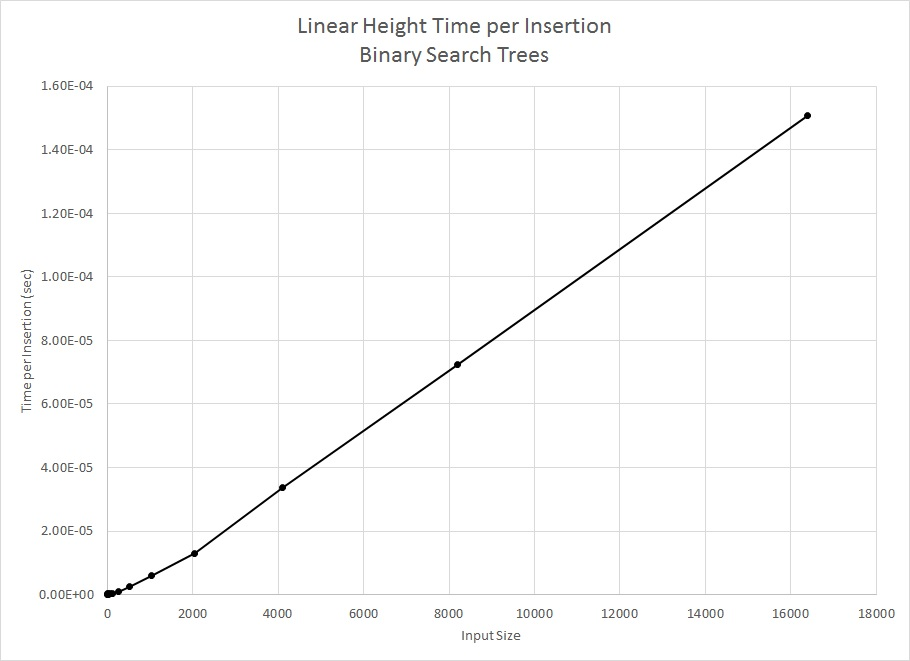
\includegraphics[width=11cm]{report/Linear_Time_Per_(Binary)} \caption{Graph of the Time Taken per Addition for Different Input Sizes for
a Linear Order Added Binary Search Tree}
\label{fig:Linear_Time_Per_Binary} 
\end{figure}


\begin{figure}[h]
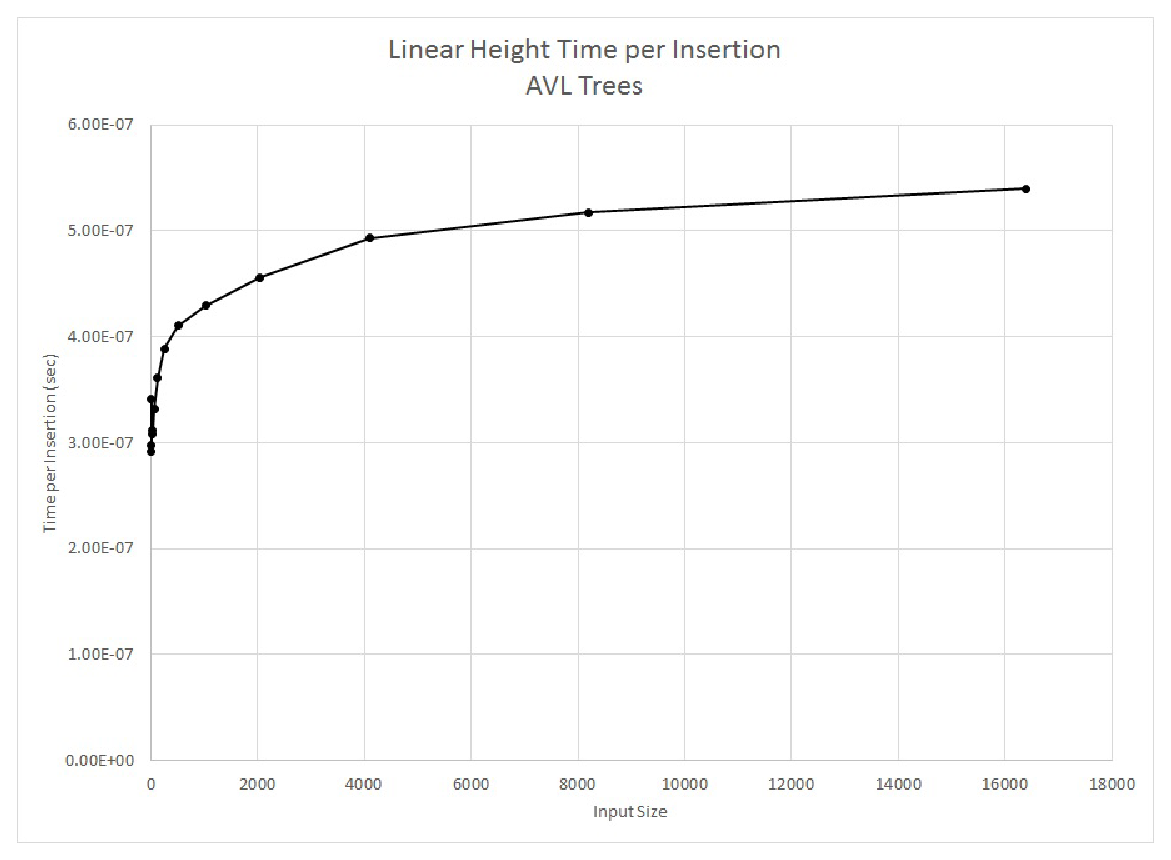
\includegraphics[width=11cm]{report/Linear_Time_Per_(AVL)} \caption{Graph of the Time Taken for Different Input Sizes for a Linear Order
Added AVL Tree}
\label{fig:Linear_Time_Per_AVL} 
\end{figure}


\begin{figure}[h]
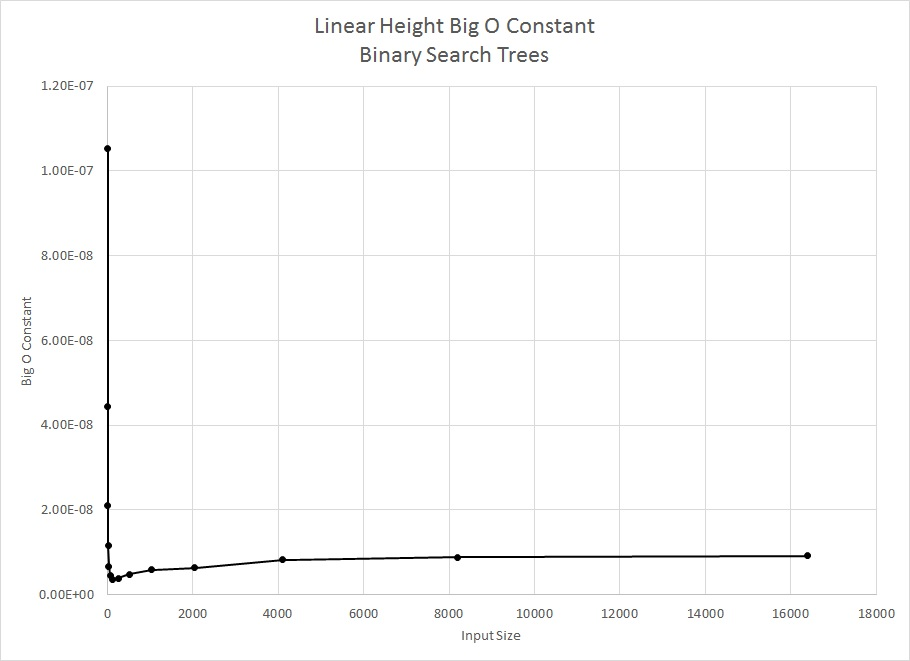
\includegraphics[width=11cm]{report/Linear_Big_O_(Binary)} \caption{Graph of the Big O Constants for Different Input Sizes for a Linear
Order Added Binary Search Tree}
\label{fig:Linear_Big_O_Binary} 
\end{figure}


\begin{figure}[h]
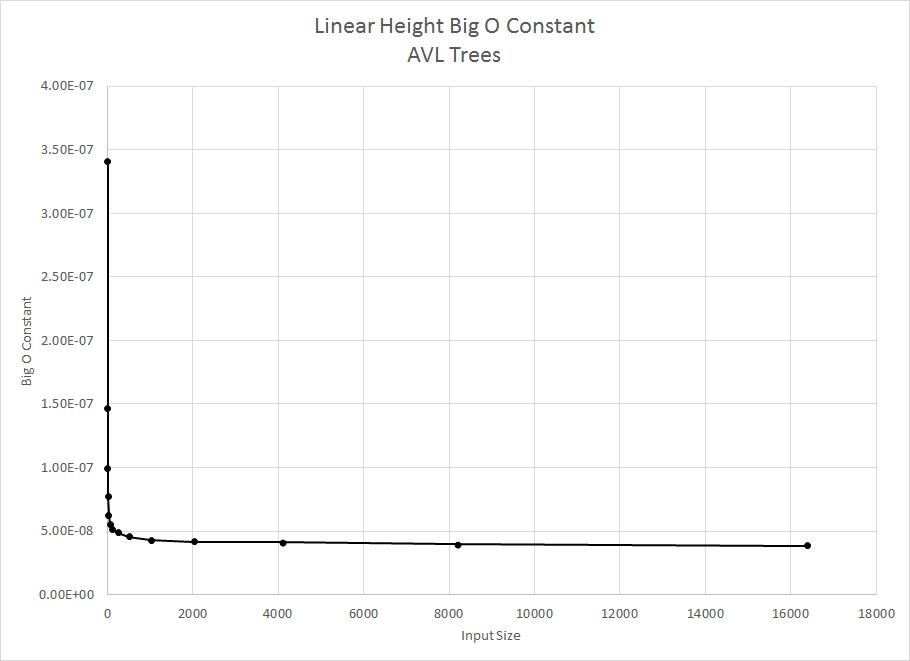
\includegraphics[width=11cm]{report/Linear_Big_O_(AVL)} \caption{Graph of the Big O Constants for Different Input Sizes for a Linear
Order Added AVL Tree}
\label{fig:Linear_Big_O_AVL} 
\end{figure}


\begin{figure}[h]
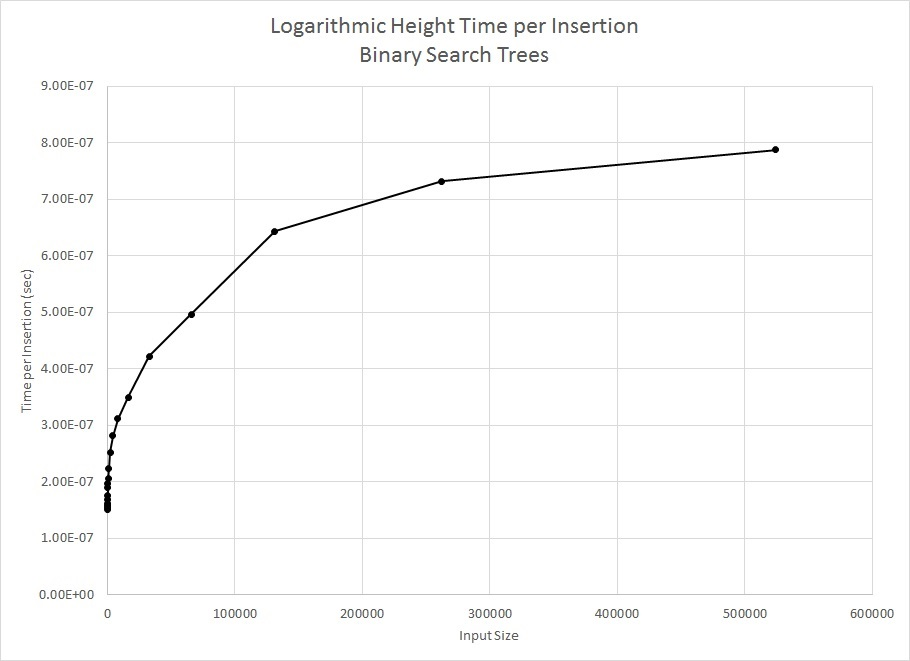
\includegraphics[width=11cm]{report/Logarithmic_Time_Per_(Binary)}
\caption{Graph of the Time Taken per Addition for Different Input Sizes for
a Logarithmic Order Added Binary Search Tree}
\label{fig:Logarithmic_Time_Per_Binary} 
\end{figure}


\begin{figure}[h]
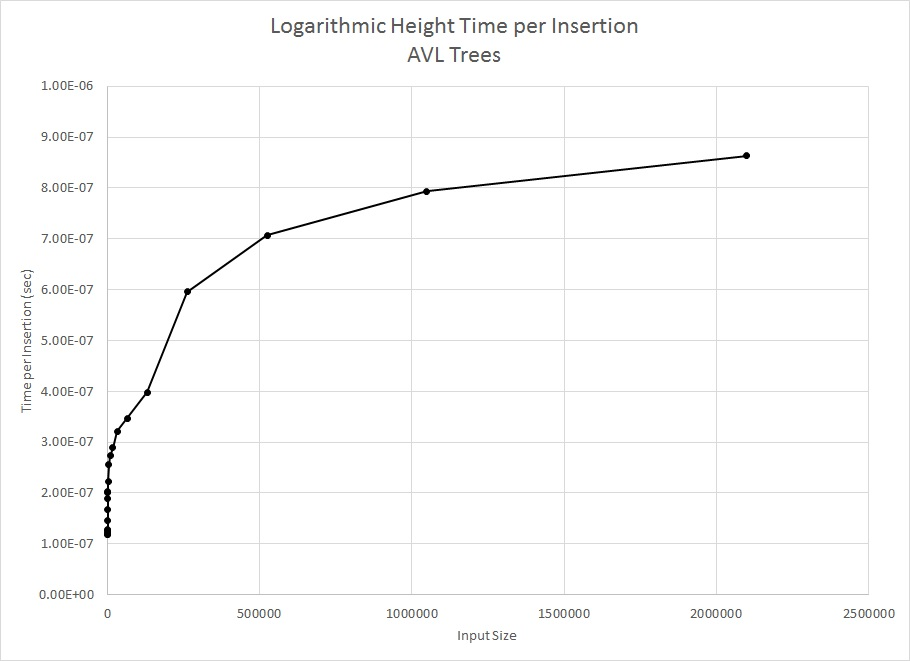
\includegraphics[width=11cm]{report/Logarithmic_Time_Per_(AVL)} \caption{Graph of the Time Taken for Different Input Sizes for a Logarithmic
Order Added AVL Tree}
\label{fig:Logarithmic_Time_Per_AVL} 
\end{figure}


\begin{figure}[h]
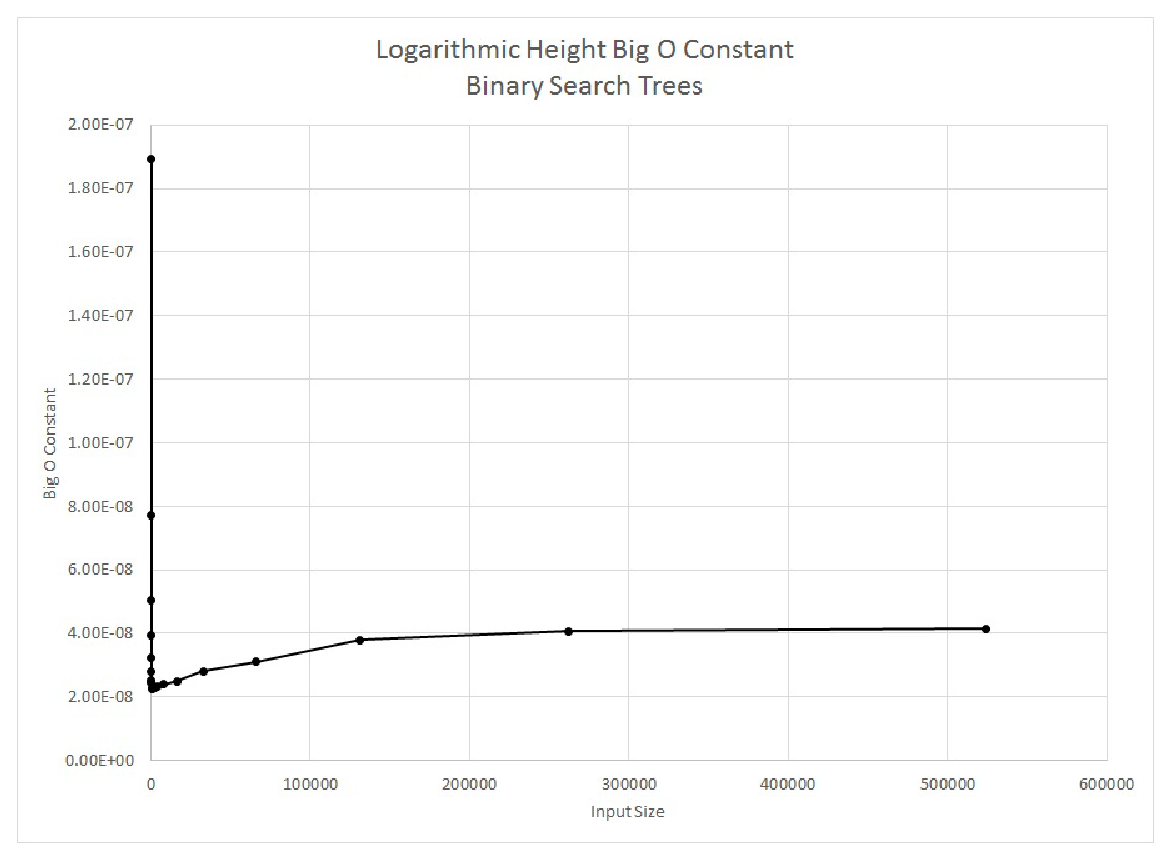
\includegraphics[width=11cm]{report/Logarithmic_Big_O_(Binary)} \caption{Graph of the Big O Constants for Different Input Sizes for a Logarithmic
Order Added Binary Search Tree}
\label{fig:Logarithmic_Big_O_Binary} 
\end{figure}


\begin{figure}[h]
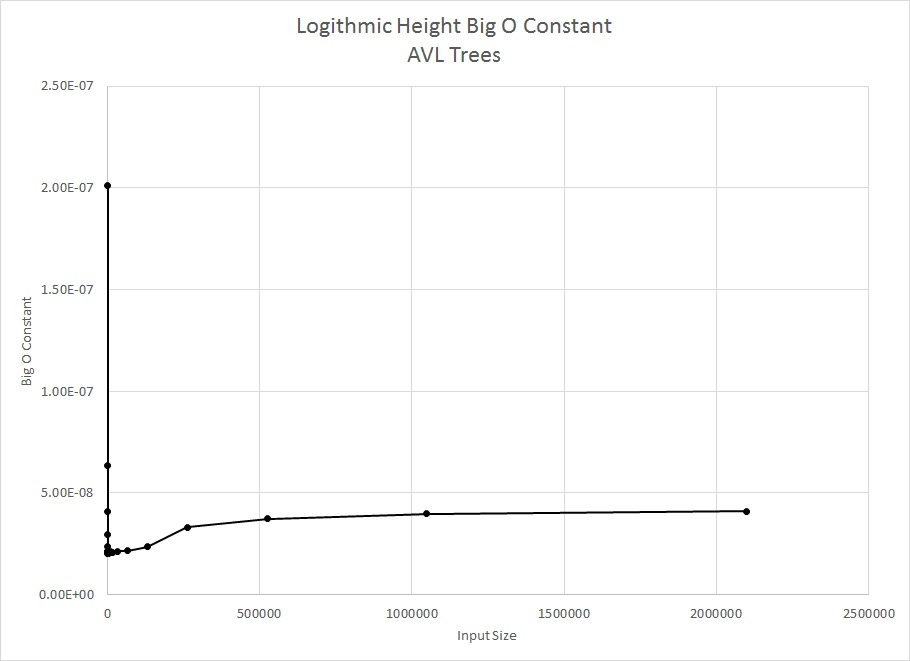
\includegraphics[width=11cm]{report/Logarithmic_Big_O_(AVL)} \caption{Graph of the Big O Constants for Different Input Sizes for a Logarithmic
Order Added AVL Tree}
\label{fig:Logarithmic_Big_O_AVL} 
\end{figure}


\begin{figure}[h]
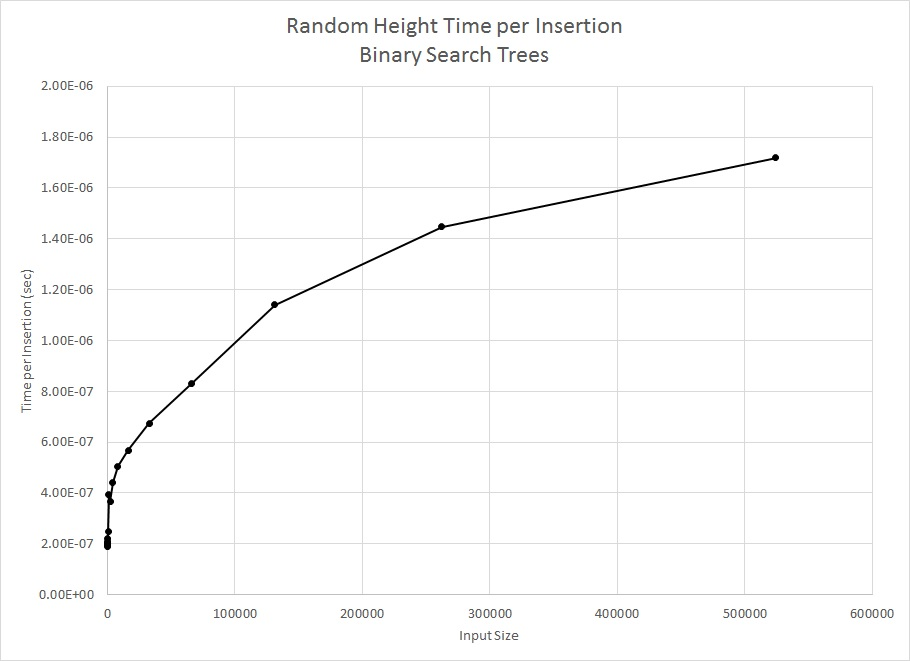
\includegraphics[width=11cm]{report/Random_Time_Per_(Binary)} \caption{Graph of the Time Taken per Addition for Different Input Sizes for
a Random Order Added Binary Search Tree}
\label{fig:Random_Time_Per_Binary} 
\end{figure}


\begin{figure}[h]
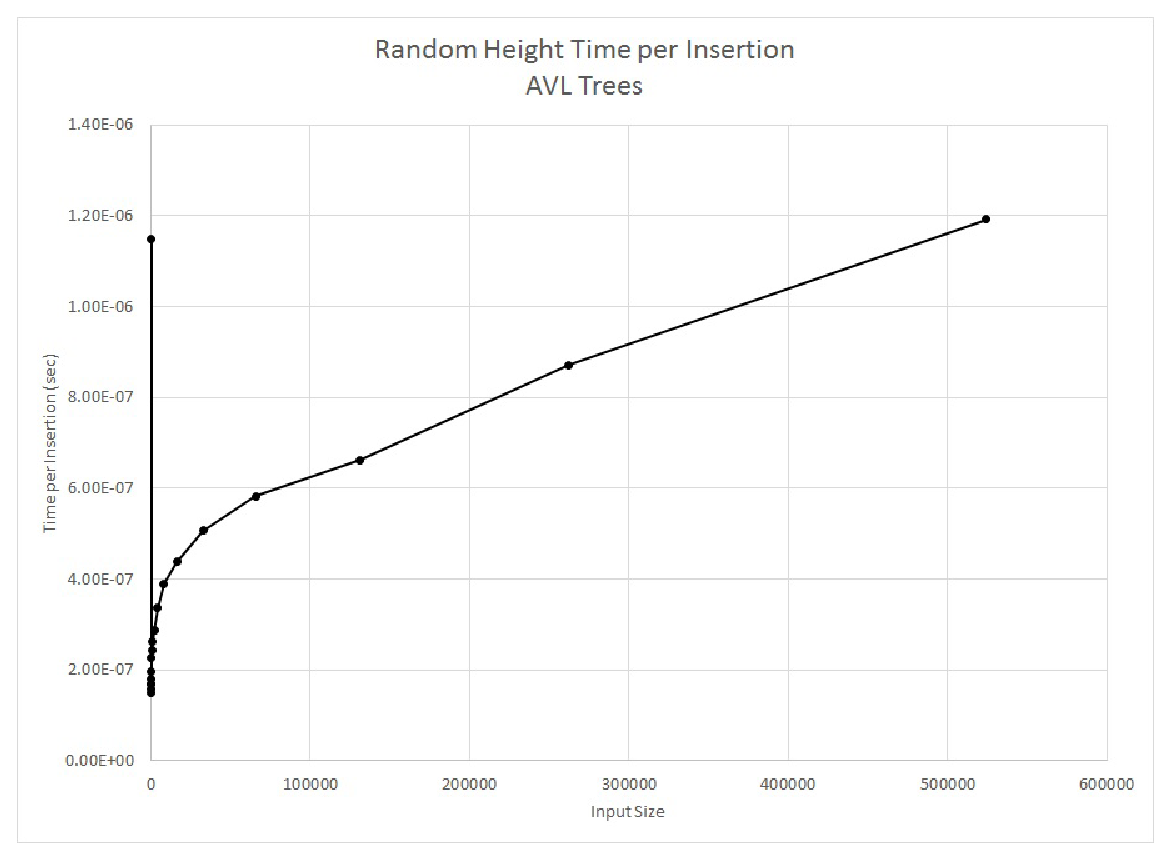
\includegraphics[width=11cm]{report/Random_Time_Per_(AVL)} \caption{Graph of the Time Taken for Different Input Sizes for a Random Order
Added AVL Tree}
\label{fig:Random_Time_Per_AVL} 
\end{figure}


\begin{figure}[h]
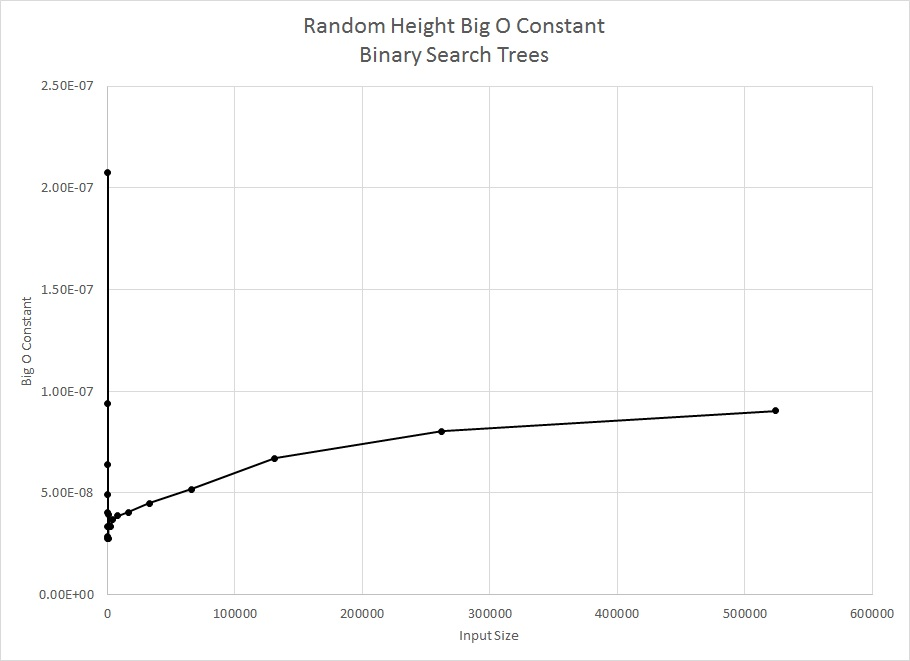
\includegraphics[width=11cm]{report/Random_Big_O_(Binary)} \caption{Graph of the Big O Constants for Different Input Sizes for a Random
Order Added Binary Search Tree}
\label{fig:Random_Big_O_Binary} 
\end{figure}


\begin{figure}[h]
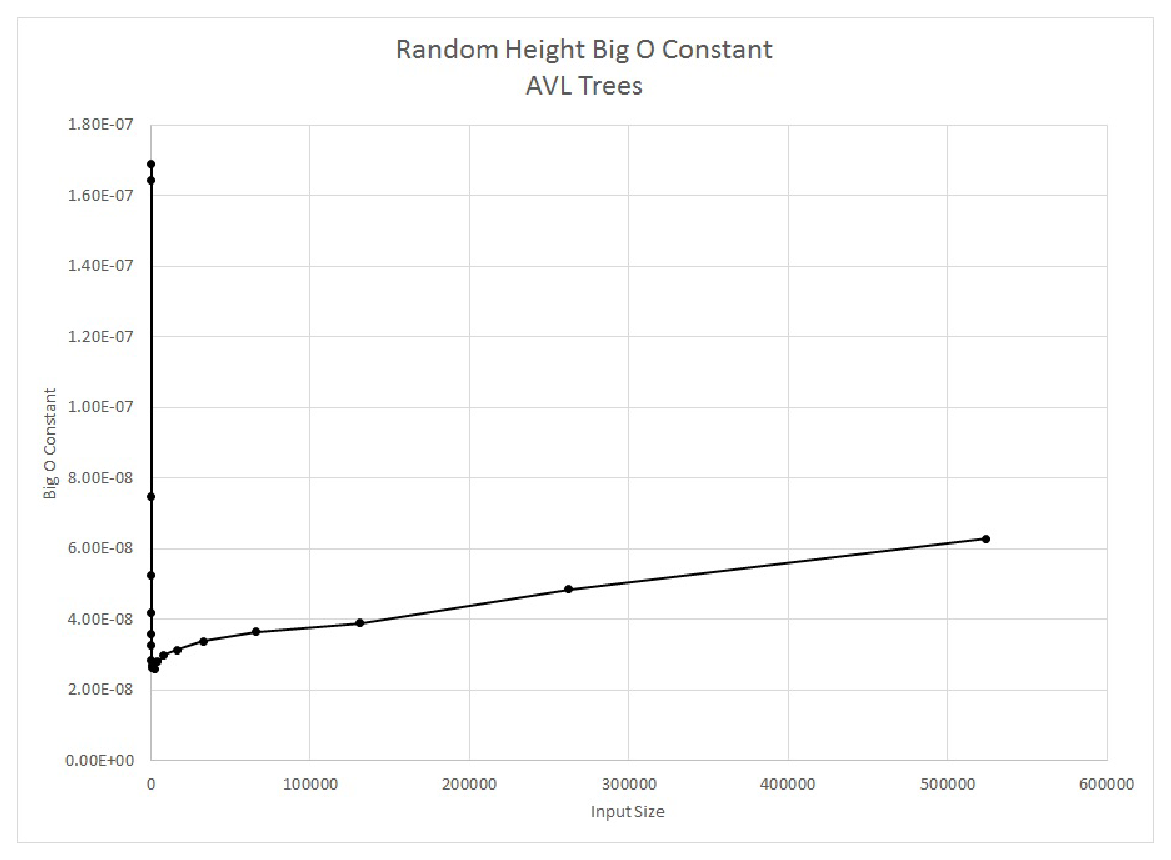
\includegraphics[width=11cm]{report/Random_Big_O_(AVL)} \caption{Graph of the Big O Constants for Different Input Sizes for a Random
Order Added AVL Tree}
\label{fig:Random_Big_O_AVL} 
\end{figure}



\section*{Conclusion}
\end{document}
